
\pdfminorversion=4 % for acroread
\documentclass[aspectratio=169,t,xcolor={usenames,dvipsnames}]{beamer}
%\documentclass[t,handout,xcolor={usenames,dvipsnames}]{beamer}
\usepackage{../beamerstyle}
\usepackage{dsfont}
\usepackage{bm}
\usepackage[english]{babel}
\usepackage[utf8]{inputenc}
\usepackage{graphicx}
\usepackage{algorithm}
\usepackage[ruled,vlined,algo2e,linesnumbered]{algorithm2e}
%\usepackage[boxed,vlined]{algorithm2e}
\usepackage{hyperref}
\usepackage{booktabs}
\usepackage{mathtools}

\usepackage{amsmath,amssymb}
\usepackage{listings}
\lstset{frame=lines,framesep=3pt,numbers=left,numberblanklines=false,basicstyle=\ttfamily\small}

\usepackage{subfig}
\usepackage{multicol}
%\usepackage{appendixnumberbeamer}
%
\usepackage{tcolorbox}

\usepackage{pgfplots}
\usepackage{tikz}
\usetikzlibrary{trees} 
\usetikzlibrary{shapes.geometric}
\usetikzlibrary{positioning,shapes,shadows,arrows,calc,mindmap}
\usetikzlibrary{positioning,fadings,through}
\usetikzlibrary{decorations.pathreplacing}
\usetikzlibrary{intersections}
\usetikzlibrary{positioning,fit,calc,shadows,backgrounds}
\pgfdeclarelayer{background}
\pgfdeclarelayer{foreground}
\pgfsetlayers{background,main,foreground}
\tikzstyle{activity}=[rectangle, draw=black, rounded corners, text centered, text width=8em]
\tikzstyle{data}=[rectangle, draw=black, text centered, text width=8em]
\tikzstyle{myarrow}=[->, thick, draw=black]

% Define the layers to draw the diagram
\pgfdeclarelayer{background}
\pgfdeclarelayer{foreground}
\pgfsetlayers{background,main,foreground}

%\usepackage{listings}
%\lstset{numbers=left,
%  showstringspaces=false,
%  frame={tb},
%  captionpos=b,
%  lineskip=0pt,
%  basicstyle=\ttfamily,
%%  extendedchars=true,
%  stepnumber=1,
%  numberstyle=\small,
%  xleftmargin=1em,
%  breaklines
%}

 
\definecolor{blue}{RGB}{0, 74, 153}

\usetheme{Boadilla}
%\useinnertheme{rectangles}
\usecolortheme{whale}
\setbeamercolor{alerted text}{fg=blue}
\useoutertheme{infolines}
\setbeamertemplate{navigation symbols}{\vspace{-5pt}} % to lower the logo
\setbeamercolor{date in head/foot}{bg=blue} % blue
\setbeamercolor{date in head/foot}{fg=white}
\setbeamercolor{author in head/foot}{bg=blue} %blue
\setbeamercolor{title in head/foot}{bg=blue} % blue
\setbeamercolor{title}{fg=white, bg=blue}
\setbeamercolor{block title}{fg=white,bg=blue}
\setbeamercolor{block body}{bg=blue!10}
\setbeamercolor{frametitle}{fg=white, bg=blue}
\setbeamercovered{invisible}

\makeatletter
\setbeamertemplate{footline}
{
  \leavevmode%
  \hbox{%
  \begin{beamercolorbox}[wd=.333333\paperwidth,ht=2.25ex,dp=1ex,center]{author in head/foot}%
    \usebeamerfont{author in head/foot}\insertshortauthor
  \end{beamercolorbox}%
  \begin{beamercolorbox}[wd=.333333\paperwidth,ht=2.25ex,dp=1ex,center]{title in head/foot}%
    \usebeamerfont{title in head/foot}\insertshorttitle
  \end{beamercolorbox}%
  \begin{beamercolorbox}[wd=.333333\paperwidth,ht=2.25ex,dp=1ex,right]{date in head/foot}%
    \usebeamerfont{date in head/foot}Week \@week, Topic \@topicnumber, Slide \insertframenumber{}\hspace*{2em}
%    \insertframenumber\hspace*{2ex} 
  \end{beamercolorbox}}%
  \vskip0pt%
}

\newcommand{\@week}{0}
\newcommand{\@topicnumber}{0}
\newcommand{\week}[1]{\renewcommand{\@week}{#1}}
\newcommand{\topicnumber}[1]{\renewcommand{\@topicnumber}{#1}}

\makeatother

%\pgfdeclareimage[height=1.2cm]{automl}{images/logos/automl.png}
%\pgfdeclareimage[height=1.2cm]{freiburg}{images/logos/freiburg}

%\logo{\pgfuseimage{freiburg}}

\input{../latex_main/macros}






\title[AutoML: Risks]{AutoML: Evaluation} % week title
\subtitle{Evaluation of ML Models (Review)} % video title
\author[Lars Kotthoff]{\underline{Bernd Bischl} \and Frank Hutter \and \underline{Lars Kotthoff}\newline \and Marius Lindauer \and Joaquin Vanschoren}
\institute{}
\date{}
\week{2}
\topicnumber{2}

\newcommand\reffootnote[1]{%
    \begingroup
    \renewcommand\thefootnote{}\footnote{
        \tiny #1
    \vspace*{1em}}%
    \addtocounter{footnote}{-1}%
    \endgroup
}

% \AtBeginSection[] % Do nothing for \section*
% {
%   \begin{frame}{Outline}
%     \bigskip
%     \vfill
%     \tableofcontents[currentsection]
%   \end{frame}
% }

\begin{document}
	
	\maketitle

    \begin{frame}[c]{Introduction}
    \begin{description}
    \item[Performance estimation of a model]
        Estimate generalization error of a model on new (unseen) data, drawn from the same data generating process.
    \item[Performance estimation of an algorithm]
        Estimate generalization error of a learning algorithm, trained on a data set
        of a certain size, on new (unseen) data, all drawn from the same data generating process.
    \item[Model selection]
        Select the best model from a set of potential candidate models (e.g., different model classes, different
        hyperparameter settings, different feature sets).
    \end{description}
    \end{frame}

    \begin{frame}[c]{Performance Evaluation}
    ML performance evaluation provides clear and simple protocols for reliable model
    validation. 

    \begin{itemize}
    \item often simpler than classical statistical model diagnosis
    \item relies only on few assumptions
    \item still hard enough and offers \textbf{lots} of options to cheat and make mistakes
    \end{itemize}
    \end{frame}

    \begin{frame}[c]{Performance Measures}

    We measure performance using a statistical estimator for the 
    \textbf{generalization error} (GE).

    $\text{GE} = $ expected loss of a fixed model

    $\hat{\text{GE}} = $ estimated loss averaged across finite sample

    Example: Mean squared error (L2 loss)
    \[
        \hat{\text{GE}} = MSE = \frac{1}{n} \sum_{i=1}^n \left(\yI{i} - \hat{y}^{(i)}\right)^2
    \]

    \end{frame}

    \begin{frame}[c]{Measures: Inner vs.\ Outer Loss}

    \begin{center}
        Inner loss = loss used in learning (training)\\
        Outer loss = loss used in evaluation (testing)\\
            = evaluation measure
    \end{center}

    Optimally: inner loss = outer loss\\[.5em]
    Not always possible:\\ some losses are hard to optimize or no loss is specified directly\\
    
    \bigskip

    Example:\\[.5em]
    \begin{tabular}{ll}
    Logistic Regression & $\rightarrow$ minimize binomial loss \\
    kNN & $\rightarrow$ no explicit loss minimization\\
    \end{tabular}

    \end{frame}

    \begin{frame}[c,allowframebreaks]{Inner Loss Example: Polynomial Regression}

    Sample data from sinusoidal function
    $0.5 + 0.4 \cdot \sin (2 \pi x) + \epsilon$
    with measurement error $\epsilon$.

    \begin{center}
    \includegraphics[width=.7\textwidth]{poly}
    \end{center}

    Assume data generating process unknown. Approximate with $d$th-degree polynomial:
    \[ f(\mathbf{x} | \mathbf{\theta}) = \theta_0 + \theta_1 x + \cdots + \theta_d x^d = \sum_{j = 0}^{d} \theta_j x^j \]

    \framebreak

    How should we choose $d$?

    \begin{center}
    \includegraphics[width=.5\textwidth]{poly-train}
    \end{center}

    d=1: MSE = 0.036 -- clear underfitting, d=3: MSE = 0.003 -- ok?, d=9: MSE =
    0.001 -- clear overfitting

    Simply using the training error seems to be a bad idea.

    \end{frame}

    \begin{frame}[c,allowframebreaks]{Outer Loss Example: Polynomial Regression}

    \begin{center}
    \includegraphics[width=.7\textwidth]{polyt}
    \end{center}

    \framebreak

    How should we choose $d$?

    \begin{center}
    \includegraphics[width=.5\textwidth]{poly-test}
    \end{center}

    d=1: MSE = 0.038 -- clear underfitting, d=3: MSE = 0.002 -- ok?, d=9: MSE =
    0.046 -- clear overfitting

    \framebreak

    \begin{center}
    \includegraphics[width=.9\textwidth]{bias-variance}
    \end{center}

    \end{frame}

    \begin{frame}[c]{General Trade-Off Between Error and Complexity}
    \includegraphics[width=\textwidth]{overfitting}
    \end{frame}

    \begin{frame}[c]{Resampling}
        \begin{itemize}
            \item uses data efficiently
            \item repeatedly split in train and test, average results
            \item make training sets large (to keep the pessimistic bias small),
                reduce variance introduced by smaller test sets through many
                repetitions and averaging of results
        \end{itemize}
    \end{frame}

    \begin{frame}[c]{Cross-Validation}

    \begin{itemize}
      \item split data into $k$ roughly equally-sized partitions
      \item use each part as test set and join the $k-1$ others for training,
          repeat for all $k$ combinations
      \item obtain $k$ test errors and average
    \end{itemize}

    Example 3-fold cross-validation:

    \begin{center}
    % FIGURE SOURCE: https://docs.google.com/presentation/d/1sKtnj5nIQrcOGU7rTisMsppUGOk7UX2gbjKhtQmTX7g/edit?usp=sharing
    \includegraphics[height=.5\textheight]{crossvalidation.png}
    \end{center}
    10-fold cross-validation is common.
    \end{frame}

    \begin{frame}[c]{Bootstrap}

        \begin{itemize}
          \item randomly draw $k$ training sets of size $n$ with replacement
                from the data
          \item evaluate on observations from the original data that are not in
              the training set
          \item obtain $k$ test errors and average
        \end{itemize}

    \begin{center}
    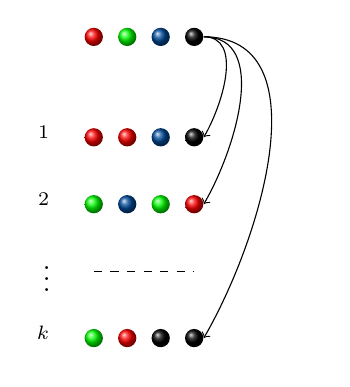
\begin{tikzpicture}[scale=1.7]
    % style
    \tikzstyle{rboule} = [circle,scale=0.7,ball color=red]
    \tikzstyle{gboule} = [circle,scale=0.7,ball color=green]
    \tikzstyle{bboule} = [circle,scale=0.7,ball color=blue]
    \tikzstyle{nboule} = [circle,scale=0.7,ball color=black]
    \tikzstyle{sample} = [->,thin]

    % title initial sample
    \path (3.5,3.75) node[anchor=east] {$\datasettrain$};

    % labels
    \path (3.5,3)   node[anchor=east] {$\datasettrain^1$};
    \path (3.5,2.5) node[anchor=east] {$\datasettrain^2$};
    \path (3.5,1.5) node[anchor=east] {$\datasettrain^k$};

    \path (3.5,2) node[anchor=east] {$\vdots$};
    \path[draw,dashed] (3.75,2.0) -- (4.5,2.0);

    % initial sample
    \path ( 3.75,3.75) node[rboule] (j01) {};
    \path ( 4.00,3.75) node[gboule] (j02) {};
    \path ( 4.25,3.75) node[bboule] (j03) {};
    \path ( 4.5,3.75) node[nboule] (j20) {};

    % bootstrap 1
    \path ( 3.75, 3.0) node[rboule] {};
    \path ( 4.00, 3.0) node[rboule] {};
    \path ( 4.25, 3.0) node[bboule] {};
    \path ( 4.5, 3.0) node[nboule] (b1) {};

    % bootstrap 2
    \path ( 3.75, 2.5) node[gboule] {};
    \path ( 4.00, 2.5) node[bboule] {};
    \path ( 4.25, 2.5) node[gboule] {};
    \path ( 4.5, 2.5) node[rboule] (b2) {};

    % bootstrap N
    \path (3.75,1.5) node[gboule] {};
    \path (4,1.5) node[rboule] {};
    \path (4.25,1.5) node[nboule] {};
    \path (4.5,1.5) node[nboule] (bN) {};

    % arrows
    \path[sample] (j20.east) edge [out=0, in=60] (b1.east);
    \path[sample] (j20.east) edge [out=0, in=60] (b2.east);
    \path[sample] (j20.east) edge [out=0, in=60] (bN.east);
    \end{tikzpicture}
    \end{center}

    Training sets will contain about 63.2\% of observations on average.

    \end{frame}    

    \begin{frame}[c,allowframebreaks]{Learning Curves}

    \begin{itemize}
    \item compares performance of a model on training and test data over a varying number of training instances $\rightarrow$ how fast can a learner learn the given relationship in the data?
    \item can also be over number of iterations of a learner (e.g.\ epochs in
        deep learning), or AutoML system over time
    \item learning usually fast in the beginning
    \item visualizes when a learner has learned as much as it can:
    \begin{itemize}
    \item when performance on training and test set reach a plateau
    \item when gap between training and test error remains the same
    \end{itemize}
    \end{itemize}

    \begin{center}
    \includegraphics[height=.35\textheight]{learning-curve}
    \end{center}

    \framebreak

    Ideal learning curve:

    \begin{center}
    \includegraphics[height=.7\textheight]{learning-curve-ideal}
    \end{center}

    \framebreak

    In general, there are two reasons for a bad learning curve:

    \begin{enumerate}
    \item high bias in model/underfitting
    \begin{itemize}
    \item training and test errors converge at a high value
    \item model can't learn underlying relationship and has high systematic errors, no matter how big the training set
    \item poor fit, which also translates to high test error
    \end{itemize}

    \begin{center}
    \includegraphics[width=.7\textwidth]{learning-curve-underfitting}
    \end{center}

    \framebreak

    \item high variance in model/overfitting
    \begin{itemize}
    \item large gap between training and test errors
    \item model requires more training data to improve
    \item model has a poor fit and does not generalize well
    \end{itemize}

    \begin{center}
    \includegraphics[width=.7\textwidth]{learning-curve-overfitting}
    \end{center}

    \end{enumerate}
    \end{frame}

\end{document}
